\niparagraph{Area overhead.}
%
The main source of area overhead in the \neupims architecture is the dual row buffer. %In the architecture of NeuPIMs, the main source of area overhead is from the dual row buffer.
%
We use CACTI 7.0~\cite{cacti-v7} with 22nm technology to measure the area overhead by doubling the row buffer resource usage in the tool configuration.
%
We observe 3.11\% area overhead, which is marginal considering the significant performance boost provided the microarchitectural addition. % Adding an additional row buffer takes up a negligible area overhead of only 3.11\%, compared to the original DRAM bank area.
%

\begin{table}[t]
\caption{\neupims power overhead.}
\footnotesize
\label{tab:power}
\vspace{-2ex}
\begin{tabular}{l|ll}
\hline
\multicolumn{1}{c|}{\textbf{Baseline}} & \multicolumn{2}{c}{\textbf{Average Power}}    \\ \hline
NPU-only                               & \multicolumn{1}{l|}{HBM (non-PIM)}         & 364.1 mW \\
\neupims                                & \multicolumn{1}{l|}{Dual row buffered PIM} & 634.8 mW \\ \hline
\end{tabular}
\vspace{-3ex}
\end{table}

%
\niparagraph{Power overhead.}
Compared to the NPU-only counterpart, \neupims requires higher power in memory because it operates NPU and PIM concurrently. 
%
We examine this power implication by measuring it using Micron's DRAM power model~\cite{micron-power} provided by DRAMsim3~\cite{dramsim3}. 
%
We assume all-bank computation command incurs 4$\times$ higher power than read command~\cite{newton}. 
%
Moreover, the ``additional'' row buffer requires DRAM to consume more background power to hold each row buffer status. 
%
We measure the total power overhead by aggregating all these factors together.  
%
Table~\ref{tab:power} compares the average power of \neupims and NPU-only system where NPUs are equipped with vanilla HBMs. 
%
\neupims exhibit 1.8$\times$ higher power consumption, offering 2.4$\times$ speedup, which can be translated into 25\% energy reduction.

\begin{figure}[t]
        \centering
        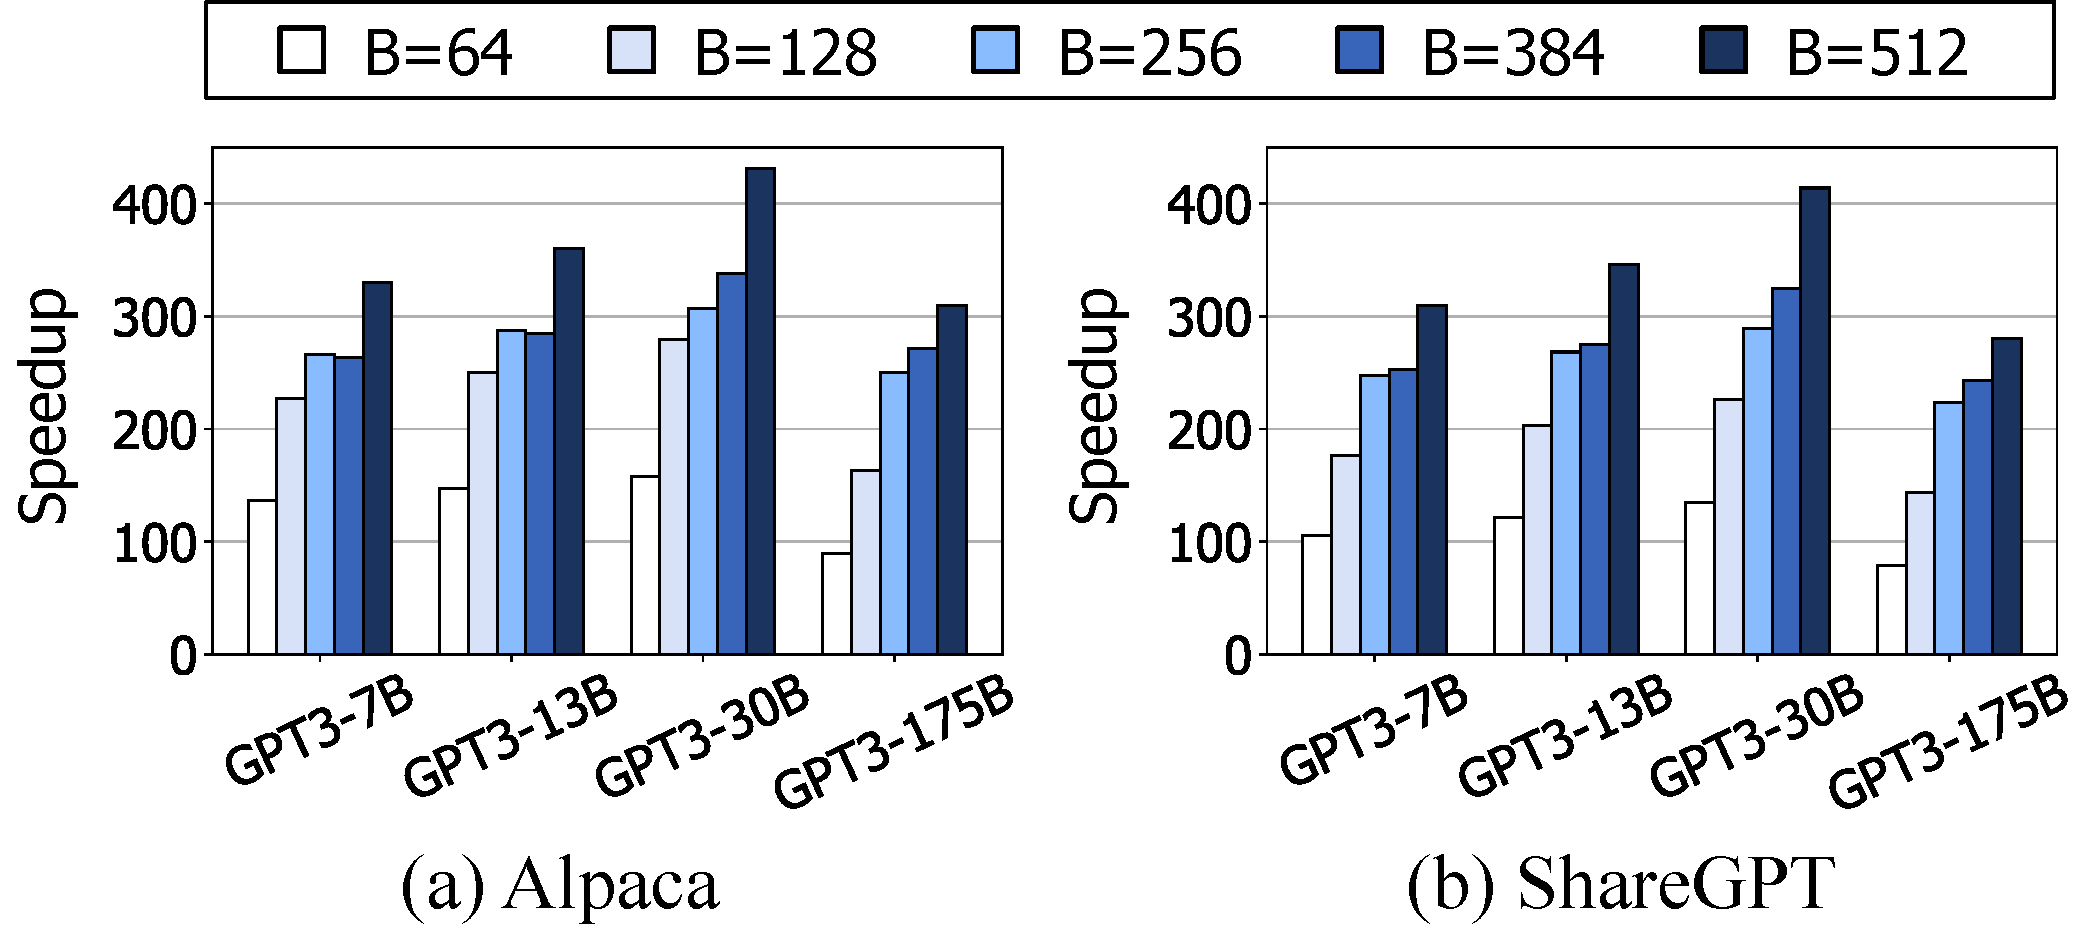
\includegraphics[width=1.0\linewidth]{figure/speedup-over-transpim.pdf}
        \vspace{-4ex}
        \caption{Speedup of \neupims over TransPIM~\cite{hpca22-transpim}.}
        \vspace{-4ex}
        \label{fig:speedup-over-transpim}
\end{figure}


\niparagraph{Comparison with TransPIM.}
TransPIM~\cite{hpca22-transpim} is a standalone PIM-only solution that operates the entirety of transformer operators within PIM devices.
%
As there is no open-source simulator for TransPIM, we develop our own TransPIM simulator based on DRAMsim3~\cite{dramsim3}.
%
We align the memory specifications of TransPIM, such as HBM timing parameters and capacity, with those used for \neupims and the NPU+PIM baseline.
%

%
Figure~\ref{fig:speedup-over-transpim} reports the speedup of \neupims over TransPIM~\cite{hpca22-transpim}
%
\neupims shows an average 228$\times$ higher throughput than TransPIM.
%
The significant performance gap is attributed to the effectiveness of GEMM computation executed on the NPU in the case of \neupims, as opposed to PIM in TransPIM.
%
That is, TransPIM specifically targets single-batch transformer model inference, making it unsuitable for batched inference. 
%
Additionally, we observe that the token-based dataflow and ring-broadcast mechanism proposed in TransPIM are designed to target encoder block operations, making them inefficient for decoder-based LLM inference.
%
Overall, \neupims consistently deliver superior performance compared to TransPIM, achieving speedups ranging from 79$\times$ to 431$\times$.
%